\documentclass[11pt]{article}
\usepackage{amsmath, amssymb,amsthm,enumerate}
\usepackage{hyperref}
\usepackage{cite}
\usepackage{geometry}
\usepackage{pdfpages}

\geometry{
 a4paper,
 total={170mm,257mm},
 left=20mm,
 top=20mm,
} 

\title{Probability Theory Homework 2}
\author{Bohao Tang}
\date{\today} 

\begin{document}
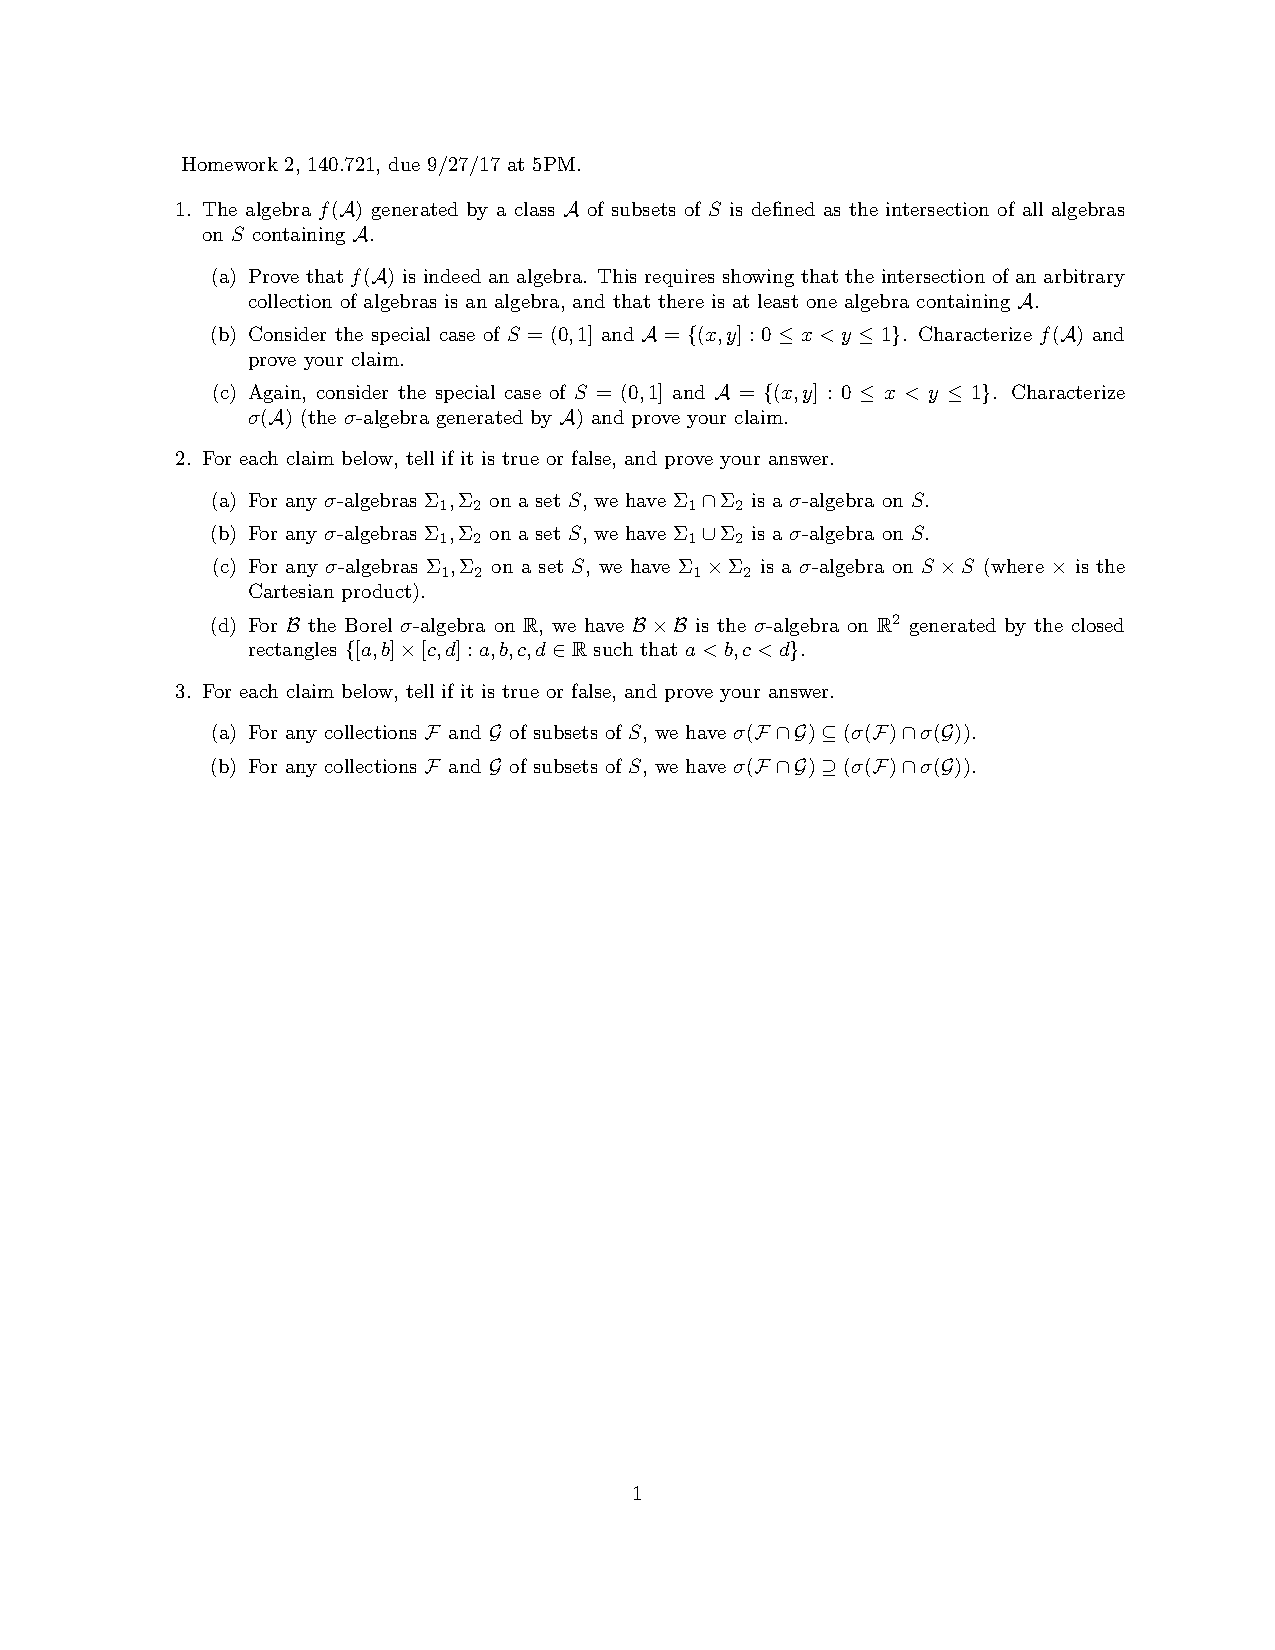
\includepdf[pages=-]{Homework2}

\maketitle

\begin{enumerate}[1.]
    \item 
    \begin{enumerate}[(a)]
        \item
        \begin{proof}
        Since the power set of $S$ is a algebra and contains $\mathcal{A}$, 
        $f(\mathcal{A})$ is well defined if the intersection of an arbitrary collection of algebras $\mathcal{A}_i, i \in I$: $\cap_{i \in I}\mathcal{A}_i$, is also an algebra.
        \begin{enumerate}[i.]
           \item
           Since $\mathcal{A}_i$ are all algebras, for all $i$: $S \in \mathcal{A}_i$, therefore $S \in \cap_{i \in I} \mathcal{A}_i$. 
           \item
           $\forall A \in \cap_{i \in I} \mathcal{A}_i$, $A$ must contains in every $\mathcal{A}_i$, then $A^c$ contains in every $\mathcal{A}_i$ because they are all algebras.
           Therefore, $A^c \in \cap_{i \in I} \mathcal{A}_i$. 
           \item
           For all $A, B$ in $\cap_{i \in I} \mathcal{A}_i$, we have $\forall i$, $A \in \mathcal{A}_i$ and $B \in \mathcal{A}_i$ $\Rightarrow$ $\forall i : A \cup B \in \mathcal{A}_i$ $\Rightarrow$ $A \cup B \in \cap_{i \in I} \mathcal{A}_i$.
        \end{enumerate}
        Therefore, $\cap_{i \in I} \mathcal{A}_i$ is indeed an algebra.
        \end{proof} 
        
        \item
        Suppose $\mathcal{C} = \{\emptyset\} \cup \{\cup_{i=1}^k (x_{2k-1}, x_{2k}] : k \in \mathbb{N}^+\ \& \ 0 \le x_1 < x_2 < x_3 < \cdots < x_{2k-1} < x_{2k} \le 1\}$.
        We prove that $f(\mathcal{A}) = \mathcal{C}$.
        \begin{proof}
            Since every element in $\mathcal{C}$ is just a finite union of sets in $\mathcal{A} \cup \{\emptyset\}$, we have $\mathcal{C} \subset f(\mathcal{A})$.
            So we only need to prove $\mathcal{C}$ is a algebra, then according to the defnition of $f(\mathcal{A})$, we have $f(\mathcal{A}) \subset \mathcal{C}$.
            And then $\mathcal{C} = f(\mathcal{A})$. Now we prove this.
            \begin{enumerate}[i.]
                \item By defnition $(0,1] \in \mathcal{C}$.
                \item For every set $A = \cup_{i=1}^k (x_{2k-1}, x_{2k}] \in \mathcal{C}$, then $A^c = C_1 \cup (x_2,x_3] \cup (x_4,x_5] \cup (x_6,x_7] \cup \cdots \cup (x_{2k-2},x_{2k-1}] \cup C_2$, where $C_1 = (0,x_1]$ if $x_1 > 0$ else $\emptyset$ and $C_2 = (x_{2k},1]$ if $x_{2k} < 1$ else $\emptyset$.
                It's easy to see that $A^c$ also obey the rules in the definition of $\mathcal{C}$.
                So $A^c \in \mathcal{C}$.
                \item For every two sets $A, B$ in $\mathcal{C}$, $A \cup B$ is a finite union of sets of form $(x,y]$, we prove now that every this kind of set is in $\mathcal{C}$.

                Suppose $W = \cup_{i=1}^n (x_i, y_i]$, then if $(x_i, y_i]$ are pairwise disjoint or $n = 1$, then we just need to put the end points in order to see that $W$ is in $\mathcal{C}$.
                If $n > 1$ and $(x_i, y_i]$ are not pairwise joint, then we can find some $(x_{i_0},y_{i_0}]$ and some $(x_{i_1},y_{i_1}],(x_{i_2},y_{i_2}], \cdots ,(x_{i_k},y_{i_k}], k \ge 1$, such that $(x_{i_0},y_{i_0}] \cap (x_{i_j},y_{i_j}] \neq \emptyset$.
                Then is easy to see that (by induction) $\cup_{j=1}^k (x_{i_j},y_{i_j}] \cup (x_{i_0},y_{i_0}] = (\min_{0\le i \le k} x_i, \max_{0\le i \le k} y_i]$. So we can replace these $k+1$ sets by one set of form $(x,y]$, where make the number of sets $n$ decrease at least $1$. 
                And we can continuously do this, since $n$ is finite. We finally will reduce $n$ to $1$ or reduce $\{(x_i,y_i]\}$ to a pairwise disjoint collection. Therefore $W$ is all in $\mathcal{C}$.

                So that $A \sup B \in \mathcal{C}$.
            \end{enumerate}
            Therefore $\mathcal{C}$ is an algebra, which ends the proof.
        \end{proof}
        
        \item
        $\sigma(\mathcal{A})$ is the Borel $\sigma$-algebra of $(0,1]$, denote it by $\mathcal{B}_{(0,1]}$.
        \begin{proof}
            For all $(x,y] \in \mathcal{A}$: If $y = 1$, $(x,1]$ is open in $(0,1]$, so $(x,1] \in \mathcal{B}_{(0,1]}$; 
            Else $(x,y] = \cap_{n=1}^\infty (x, y+\frac{1-y}{n})$.
            
            Therefore $(x,y] \in \mathcal{B}_{(0,1]} \Rightarrow \mathcal{A} \subset \mathcal{B}_{(0,1]} \Rightarrow \sigma(\mathcal{A}) \subset \mathcal{B}_{(0,1]}$

            On the other side, for all $A$ open interval relative to $(0,1]$: $A = (x,1] \in \mathcal{A}$ or $A = (x,y) = \cup_{n=1}^\infty (x,y-\frac{y-x}{n}] \in \sigma(\mathcal{A})$.
            Therefore $A \in \sigma(\mathcal{A}) \Rightarrow \mathcal{B}_{(0,1]} \subset \sigma(\mathcal{A})$.
            
            So $\sigma(\mathcal{A}) = \mathcal{B}_{(0,1]}$.
        \end{proof} 
    \end{enumerate}
    
    \item 
    \begin{enumerate}[(a)]
        \item
        True.
        \begin{proof}
            Given $\Sigma_1$ and $\Sigma_2$ be $\sigma$-algebra:
            \begin{enumerate}[i.]
                \item
                $S \in \Sigma_1$ and $S \in \Sigma_2$, so $S \in \Sigma_1 \cap \Sigma_2$.
                \item
                For all $A$ in $\Sigma_1 \cap \Sigma_2$, we have $A \in \Sigma_1$ and $A \in \Sigma_2$. 
                Therefore $A^c \in \Sigma_1$ and $\Sigma_2$ $\Rightarrow$ $A^c \in \Sigma_1 \cap \Sigma_2$.
                \item
                For all $\{A_i\}$ in $\Sigma_1 \cap \Sigma_2$, we have all $A_i$ are in $\Sigma_1$ and $\Sigma_2$. 
                Therefore $\cup_{i=1}^\infty A_i \in \Sigma_1$ and $\cup_{i=1}^\infty A_i \in \Sigma_2$ $\Rightarrow$ $\cup_{i=1}^\infty \in \Sigma_1 \cap \Sigma_2$.
            \end{enumerate}
            So, $\Sigma_1 \cap \Sigma_2$ is also $\sigma$-algebra.
        \end{proof}
        
        \item
        False.

        In $\{1,2,3,4\}$, $\{\emptyset, \{1,2\}, \{3,4\}, \{1,2,3,4\}\}$ is a $\sigma$-algebra and $\{\emptyset, \{1,3\}, \{2,4\}, \{1,2,3,4\}\}$ is a $\sigma$-algebra.
        But there union is not a $\sigma$-algebra, because $\{1,3\}$ and $\{1,2\}$ are in it but $\{1\} = \{1,3\} \cap \{1,2\}$ is not in it.
        
        \item
        False.

        If $\Sigma_1 \times \Sigma_2$ is defined by $\{A \times B \ : A \in \Sigma_1, B \in \Sigma_2\}$. Then it may not be a $\sigma$-algebra.
        For example, denote $\mathcal{B}_R$ be the Borel $\sigma$-algebra of $\mathbb{R}$. Then $\mathcal{B}_R \times \mathcal{B}_R$ contains all open rectangle. Therefore $\sigma(\mathcal{B}_R \times \mathcal{B}_R)$ is at least as large as $\mathcal{B}_{R^2}$.
        So if $\mathcal{B}_R \times \mathcal{B}_R$ is $\sigma$-algebra, then open unit circle will be in it. However, this is not the case since open cirle is not a Cartrsian product of any set. So $\mathcal{B}_R \times \mathcal{B}_R$ is not a $\sigma$-algebra.

        \item
        I think is to prove $\sigma(\left\{[a,b] \times [c,d]\right\}) = \mathcal{B}_{R^2}$. (If $\mathcal{B} \times \mathcal{B}$ is defined like in 2.c., then it will not be a $\sigma$-algebra).
        \begin{proof}
            $\mathcal{B}_{R^2}$ contains all open sets, hence it also contains all closed sets $\Rightarrow$ all $[a,b] \times [c,d] \in \mathcal{B}_{R^2} $ $\Rightarrow \sigma(\left\{[a,b] \times [c,d]\right\}) \subset \mathcal{B}_{R^2}$.
            
            On the other side we only prove that all open sets are in $\sigma(\left\{[a,b] \times [c,d]\right\})$.
            
            First, for every open rectangle $A = (a,b) \times (c,d)$: $A = \cup_{n=1}^\infty [a+\frac{b-a}{4n}, b-\frac{b-a}{4n}] \times [c+\frac{d-c}{4n}, d-\frac{d-c}{4n}]$.
            Therefore $A \in \sigma(\left\{[a,b] \times [c,d]\right\})$ $\Rightarrow \sigma(\left\{(a,b) \times (c,d)\right\}) \subset \sigma(\left\{[a,b] \times [c,d]\right\})$.

            Second, for every open set $O$, set $S = O \cap \mathbb{Q}^2$. Consider (we use $\{p,q\}$ to denote the point $(p,q) \in R^2$ and $(a,b)$ to denote open interval to avoid confusing):
            $$\mathcal{A} = \{(p,q) \times (r,s) \subset O : \{p,r\} \in S; \{q,s\} \in S\}$$
            and $D = \cup_{C \in \mathcal{A}} C$
            
            Then we have $\mathcal{A}$ is a countable collection in $\left\{(a,b) \times (c,d)\right\}$ and therefore $D \in \sigma(\left\{(a,b) \times (c,d)\right\})$.
            
            Finally, we argue that $D = O$. In the definition of $D$, we have obviously $D \subset O$. On the other hand, for every point $x = \{u,v\} \in O$, since $O$ is open, there is a open rectangle $x \in (a,b)\times(c,d) \subset O$.
            Then we have $a < u < b$ and $c < v < d$. Since $\mathbb{Q}$ is dense, we can find rational number $p,q,r,s$ such that $a<p<u<q<b$ and $c<r<v<s<d$. 
            Therefore $\{u,v\} \in (p,q)\times(r,s) \in \mathcal{A}$ $\Rightarrow \{u,v\} \in D$ $\Rightarrow O \subset D$. Therefore $D = O$.

            So every open set is in $\sigma(\left\{(a,b) \times (c,d)\right\})$ $\Rightarrow \mathcal{B}_{R^2} \subset \sigma(\left\{(a,b) \times (c,d)\right\}) \subset \sigma(\left\{[a,b] \times [c,d]\right\})$.

            Then $\mathcal{B}_{R^2} = \sigma(\left\{[a,b] \times [c,d]\right\})$.
        \end{proof}

    \end{enumerate}
    \item 
    \begin{enumerate}[(a)]
        \item
        True.
        \begin{proof}
            $\mathcal{F} \cap \mathcal{G} \subset \mathcal{F} \subset \sigma(\mathcal{F})$, and the same way we have $\mathcal{F} \cap \mathcal{G} \subset \sigma(\mathcal{G})$.
            Therefore $\mathcal{F} \cap \mathcal{G} \subset \sigma(\mathcal{F}) \cap \sigma(\mathcal{G})$. Since $\sigma(\mathcal{F}) \cap \sigma(\mathcal{G})$ is a $\sigma$-algebra (we proved it in 2.a.), we have $\sigma(\mathcal{F} \cap \mathcal{G}) \subset \sigma(\mathcal{F}) \cap \sigma(\mathcal{G})$.
        \end{proof}
        \item
        False.

        Suppose $\mathcal{F}$ is the collection of all open sets in $\mathbb{R}$ and $\mathcal{G}$ is the collection of all closed set in $\mathbb{R}$.
        Then $\sigma(\mathcal{F}) = \sigma(\mathcal{G}) = \mathcal{B}_R$. But $\sigma(\mathcal{F} \cap \mathcal{G}) = \sigma(\emptyset) \neq \mathcal{B}_R$. 
    \end{enumerate}
\end{enumerate}

\end{document}

